\documentclass[../../OAE-SPEC-MAIN.tex]{subfiles}


\title{Principles of Operation}\label{sec:principles-of-operation}

\begin{document}

\chapter{Principles of Operation}

\subfile{./section/intro.tex}

\subfile{./section/symmetric-reversibility.tex}

\subfile{./section/interactions-bandwidth.tex}

\subfile{./section/slots.tex}

\subfile{./section/promised-networks.tex}

\subfile{./section/once-delivery.tex}

\subfile{./section/counting-protocols.tex}

\subfile{./section/considerations.tex}

\end{document}







%\section{From API to Bits-on-the-wire}

%\AE thernet introduces a fundamentally new substrate for reliable communication. Every transmission is atomic, reversible, and causally consistent. To application developers, this creates the illusion of an \textit{unbreakable network}, where transactions either succeed completely or fail without side effects.

%Yet to enable adoption, \AE thernet must integrate seamlessly with existing infrastructure. The compatibility boundary is the IP layer. Above this layer, applications continue to operate as before. Below it, \AE thernet provides a drop-in replacement for traditional Ethernet, unobservable by legacy systems, but dramatically more reliable in behavior.

%However, the true potential of \AE thernet lies beyond emulation. Its atomic transaction model enables a new class of guarantees -- deterministic delivery, fault-local reversibility, and programmable transport semantics -- that cannot be expressed in the traditional IP or TCP abstractions. To expose these capabilities to applications, a new vertically integrated stack is needed.

%This stack must:
%\begin{itemize}
%\item Extend from the API boundary (e.g., sockets, RPC, shared memory transport) down to the bits on the wire.
%\item Preserve atomicity and reversibility guarantees across all abstraction layers.
%\item Offer language-level semantics (e.g., async/await, futures, or transactions) that map directly to causal protocol operations.
%\end{itemize}

%In essence, \AE thernet is not just a new physical protocol. It is a new foundation for building distributed systems, one in which software and hardware speak the same language of atomic, bidirectional flow.

%New transaction guarantees can be offered to applications, but requires a entirely new networking stack from API to bits on the wire that propagates the same guarantees of atomicity and reversibility into the languages that application developers write code with.



%\marginnote{The difference between ALOHA and slotted ALOHA is the the former requires acknowledgements, while the latter does not, assuming that the packets will get there with high reliability}

%\section{Perfect Information Feedback (PIF)}

%We use the idea of Perfect Information Feedback, from \cite{Abramson}, who described it in terms of satellite packet switching, but then abandoned positive acknowledgments because multiple receivers. he claims that a more efficient use of negative acknowledgments in conjunction with packet numbering is feasible for his system.




%\begin{marginfigure} % This is already on the previous page
%        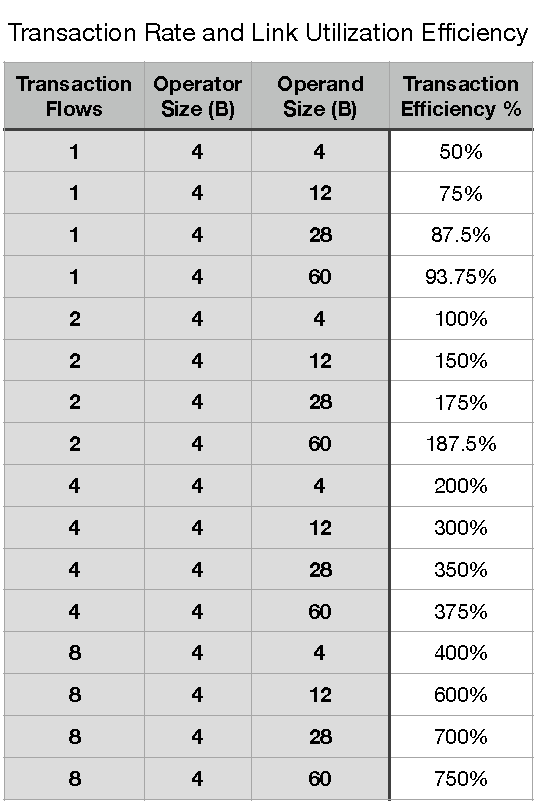
\includegraphics[width=0.92\linewidth]{.././figures/Transaction-Rate.pdf}
%  \caption{Transaction Rate Calculations}
%    \vspace{8pt}
%\end{marginfigure}



%\begin{marginfigure}
%        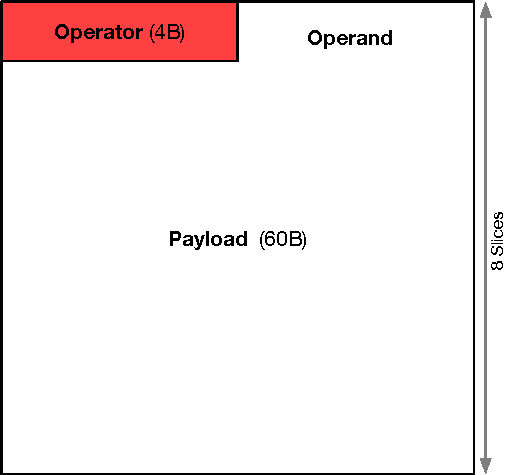
\includegraphics[width=\linewidth]{.././figures/8-slice-operator.pdf}
%  \caption{One 8 slice Flow Sub Transaction with 60B payload}
%\end{marginfigure}

%\subfile{Protocol-byte} % This is already included in the main file.

%
%\renewcommand{\bibfont}{\footnotesize}  % Footnote size for the whole bibliography
%\printbibliography

%\newpage
%\section{Virtual Channels}

%The protocol provides Endpoints for Virtual Channels. The IPV6 Format has been proposed, but this would give the false impression that the outside world (Internet) and inside world (Transaction Fabrix)/ %tm].trademark doesn't work

%\subfile{OPCODE-Byte}


